\subsection*{Four-family pharmacophore allocation study}

\input{\manuscriptroot tables/supporting-pharmacophore-mixture}

\begin{figure}[htbp]
\centering
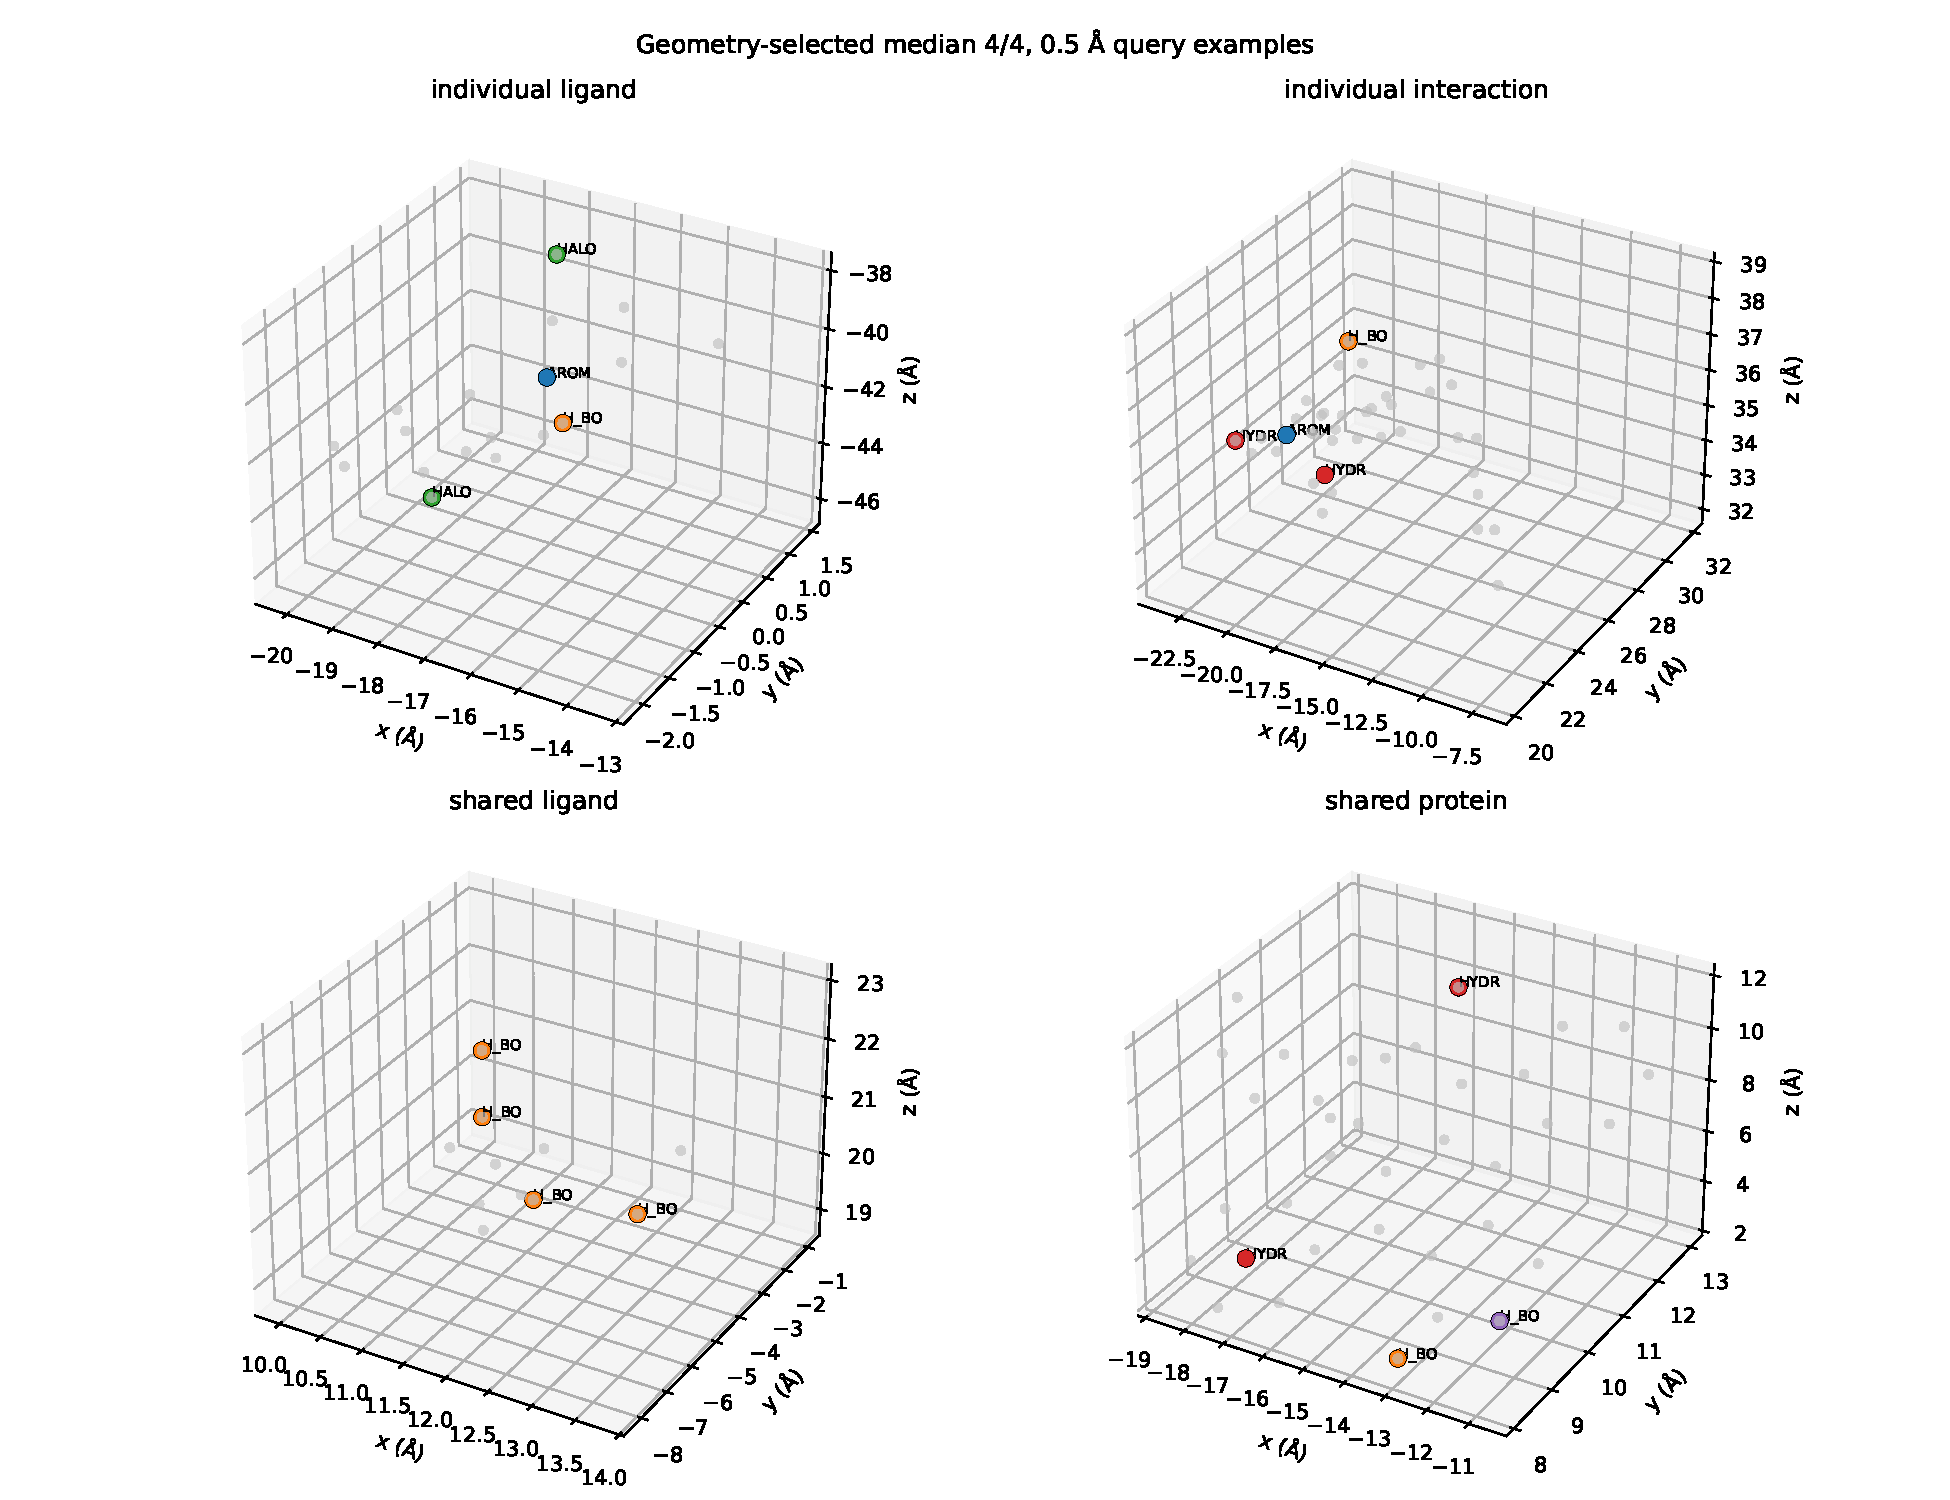
\includegraphics[width=\linewidth]{figures/supporting/cdpkit-query-family-examples.pdf}
\caption{Representative geometry-selected queries from the four CDPKit families.
Individual ligand queries use one ligand pose; individual interaction queries use
ligand features selected by one complex. Shared ligand queries retain a feature core
after ligand-feature alignment across poses. Shared protein queries retain interaction
features after pocket C$\alpha$ alignment, without subsequent feature realignment.
Examples illustrate the construction rules and were selected from reference geometry,
not generator performance.}
\label{fig:cdpkit-query-families}
\end{figure}

\begin{figure}[p]
\centering
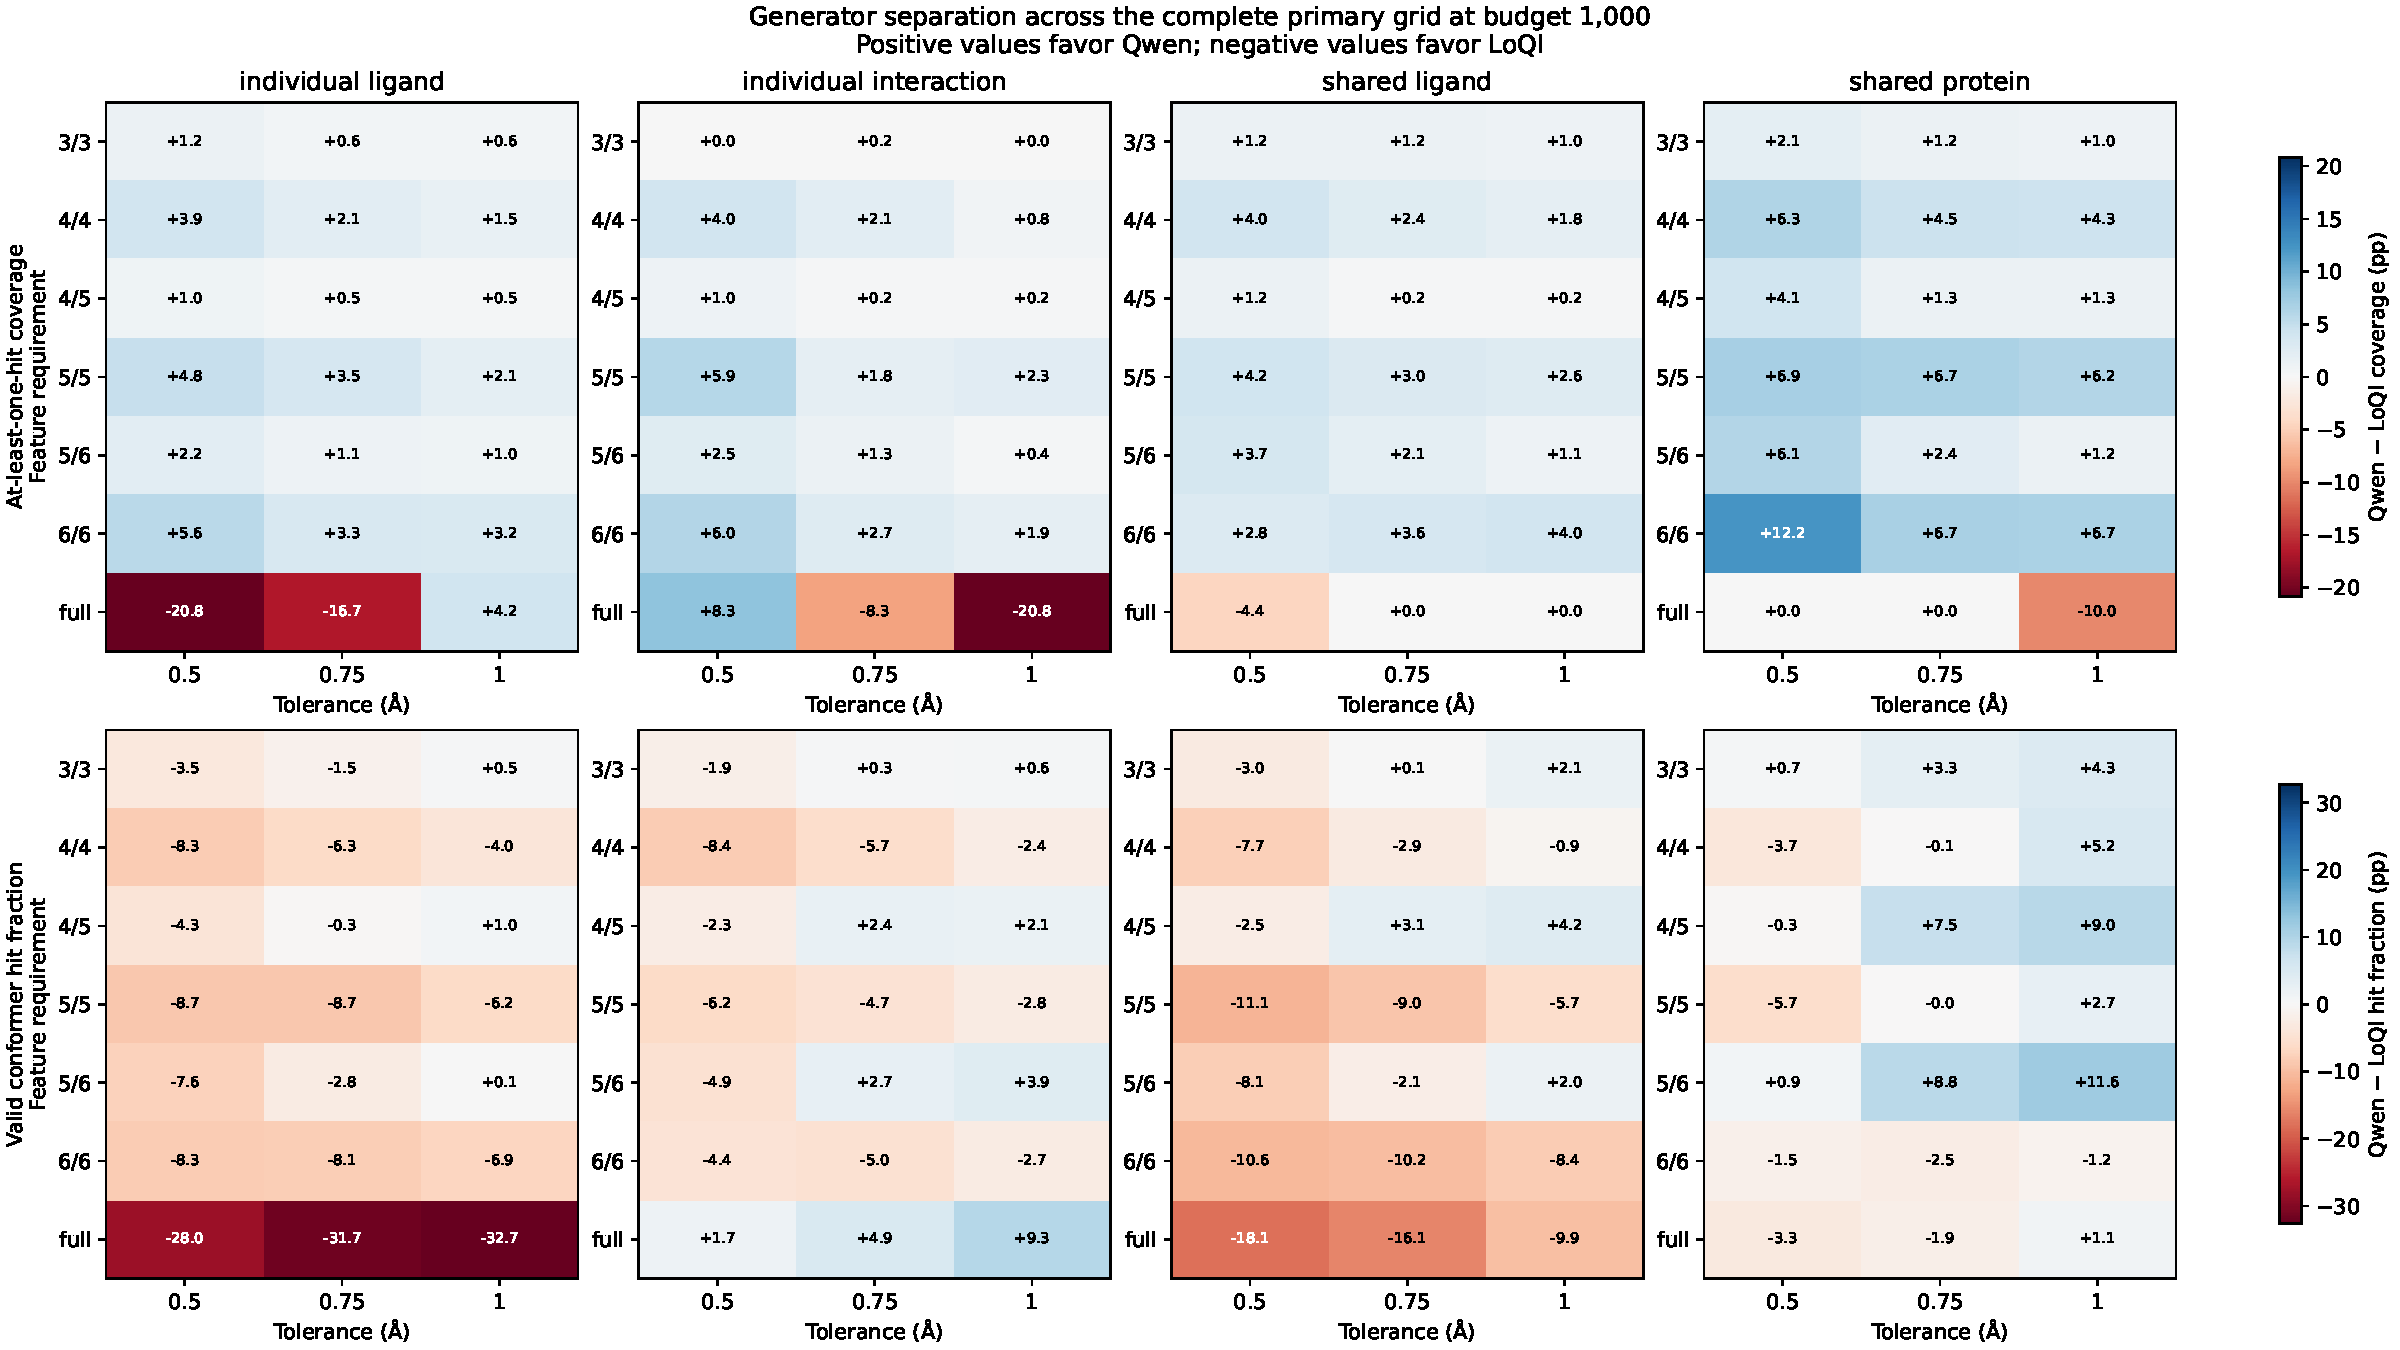
\includegraphics[width=\linewidth,height=0.82\textheight,keepaspectratio]{figures/supporting/cdpkit-generator-separation-grid.pdf}
\caption{Qwen-minus-LoQI expected coverage across the complete primary grid.
The grid contains four query families, seven feature requirements, three positional
tolerances, and four attempt budgets (336 cells). Positive values favor Qwen and
negative values favor LoQI. Cells are not independent because the same molecules,
parents, and source pools contribute to multiple settings. Displaying the complete
grid shows saturation at looser tolerances and larger budgets and prevents the main
four-of-four, 0.5~\AA{} reference comparison from being interpreted as a
result-selected query. Exploratory bootstrap intervals are not adjusted for this
grid search.}
\label{fig:cdpkit-generator-separation}
\end{figure}
